\NEW{
\section{Dynamic Bandwidth Separation}
\label{sec:dynamic}

\begin{figure}[t]
  \centering
  %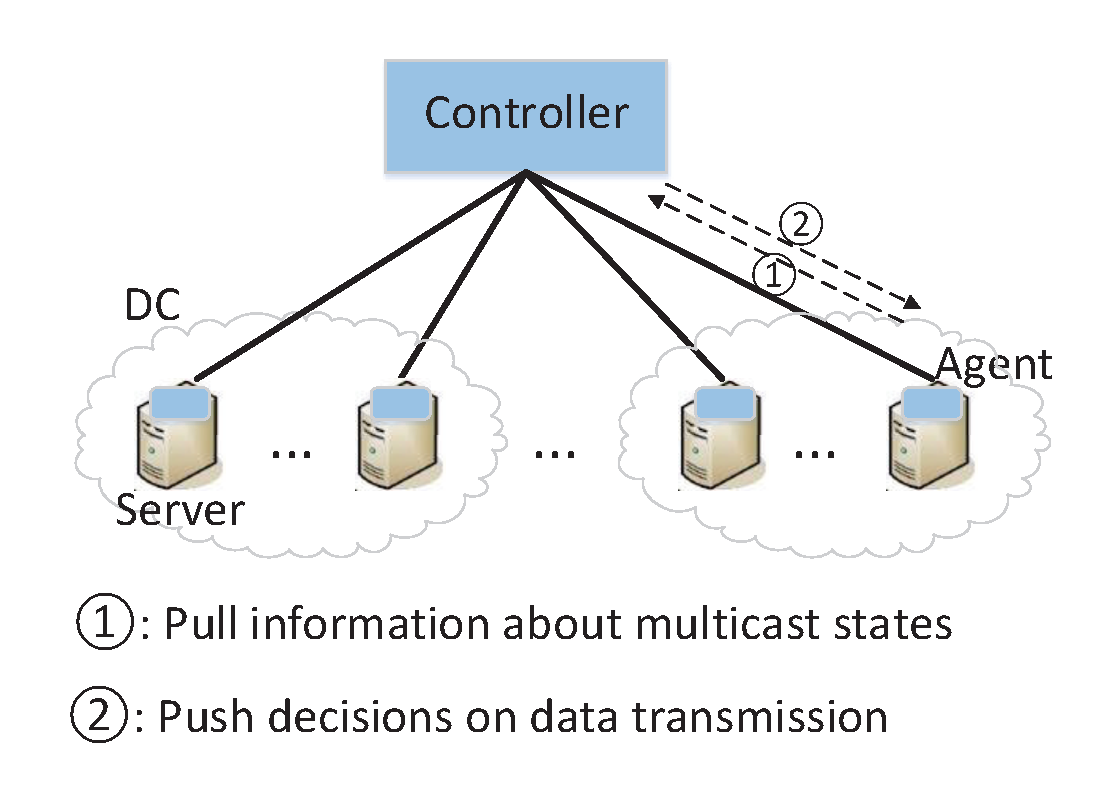
\includegraphics[width=2in]{images/framework.eps}
  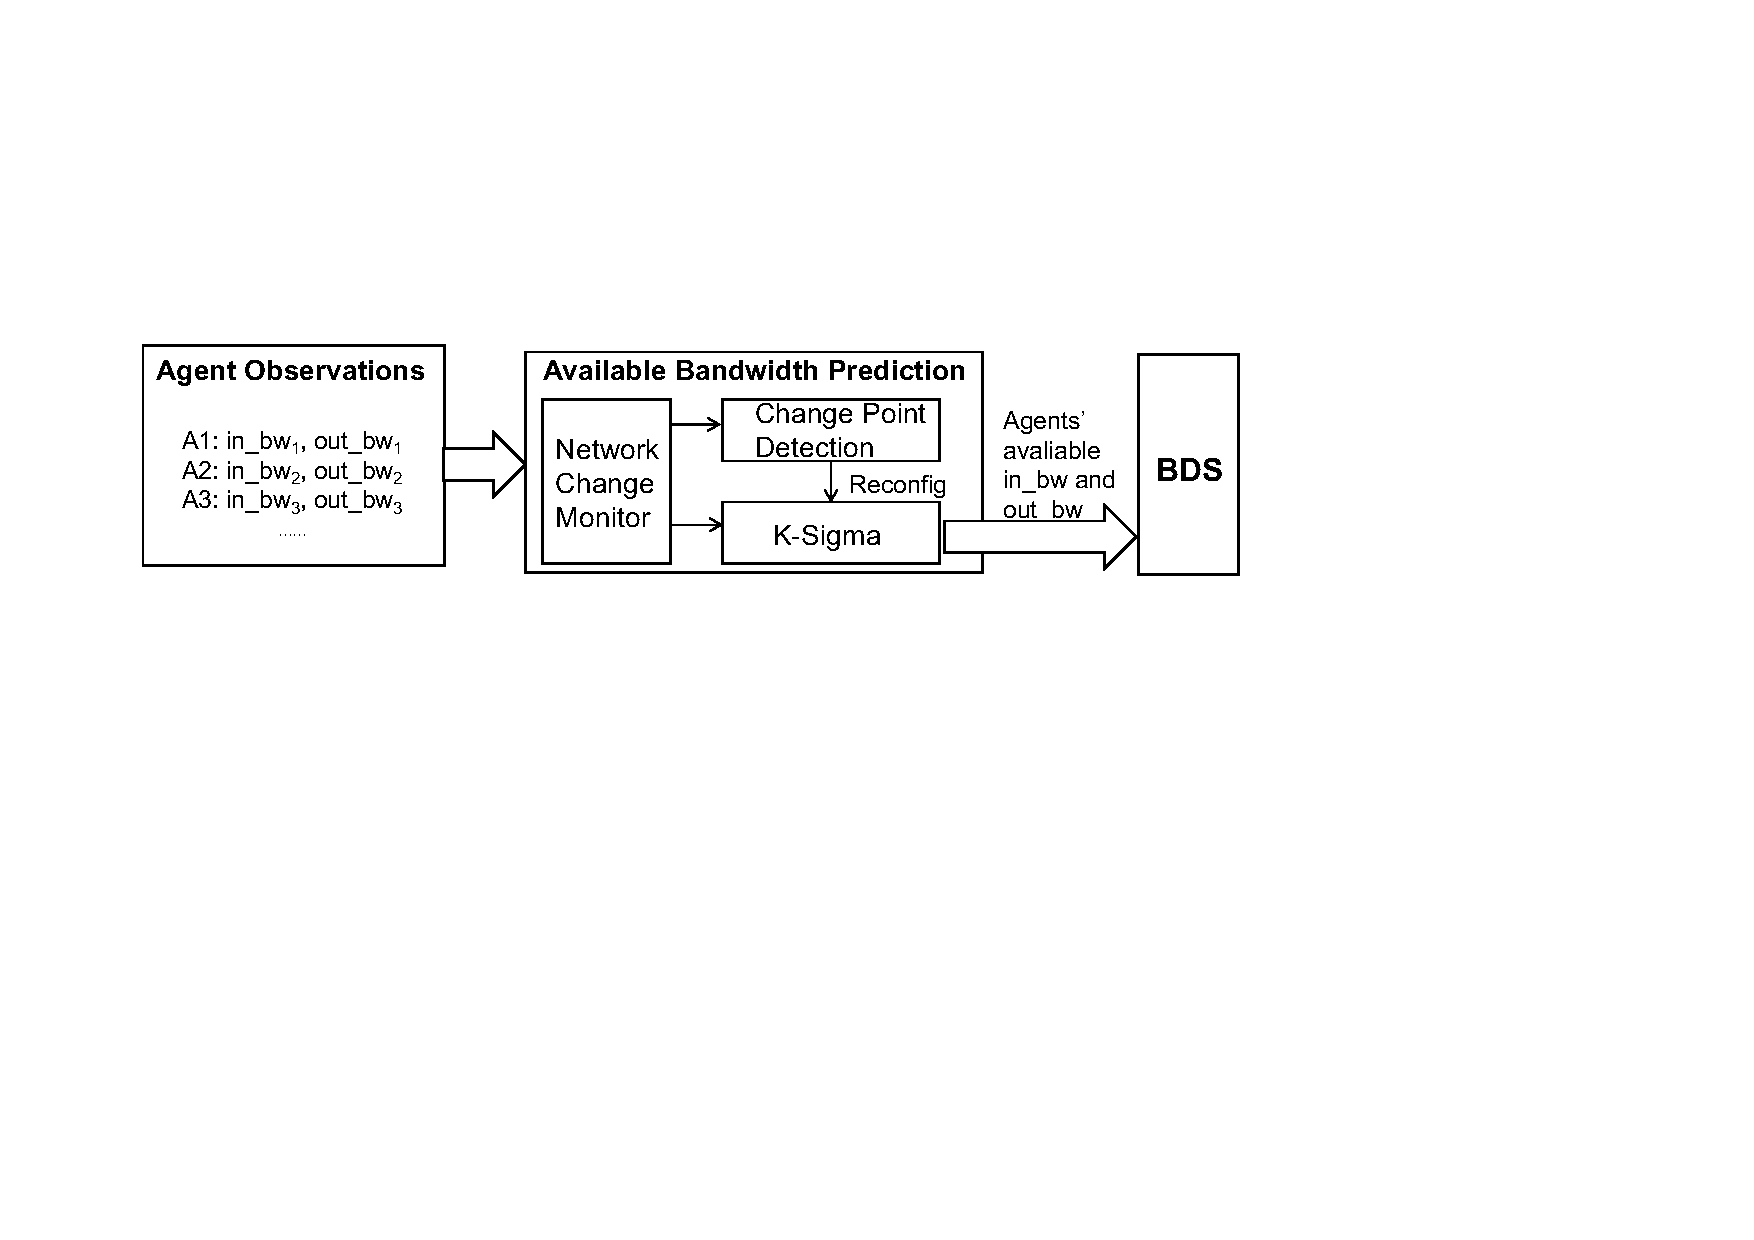
\includegraphics[width=3.4in]{images/bds+.pdf}
    \vspace{-0.2cm}
  \tightcaption{\NEW{Logical diagram of \name's dynamic bandwidth separation.}}
  \label{fig:bayes}
%\vspace{-0.4cm}
\end{figure}

\bdsname performs well under fixed network separation, but in the mixed deployment situations where online traffic and offline traffic shares the same server I/O, it results in low link utilizations when online traffic reduces. This is because bulk data transfer will never occupy any bandwidth exceeding the fixed threshold even though online traffic is far below the reserved bandwidth (see \Section\ref{subsec:motivation:baseline}).

So we further present \name with dynamic bandwidth separation, which adjusts the available bandwidth for bulk data transfer in a real-time manner, by continuously predicting online traffic and automatically adjusting the scheduling decisions, so as to fully utilize network bandwidth accordingly. To be specific, \name automatically adjust the scheduling results under different network conditions: if online traffic encounters its peak, \name shirks its occupied bandwidth to avoid congestions, while online traffic encounters its valley, \name aggressively uses more bandwidth to make full use of the residual bandwidth.

To achieve this, \name leverages a customized online traffic prediction algorithm, which identifies the changes of server bandwidth usage, and triggers re-scheduling to adjust bandwidth allocation to the bulk-data transfer. Figure~\ref{fig:bayes} shows the logical diagram of \name's dynamic bandwidth separation. The Network Change Monitor reads the agent observations ($bw_{in}$ and $bw_{out}$) and executes a customized combination of \textit{k-Sigma} \cite{ThreeSigma} and a change point detection algorithm \cite{adams2007bayesian}. \textit{k-Sigma} is responsible to calculate the mean and standard deviation of agent observation, and the change point detection is responsible for detecting abrupt changes by observing historical data, in order to make the Agent Monitor both stable and sensitive.

\minor{
To integrate to \bdsname, we make the above online traffic prediction at the beginning of each cycle, and based on the predicted traffic, \bdsname updates the available link status and then calculates bottleneck disjoint paths. As the online traffic is time-varying, the available bandwidth of all paths are therefore varies along with the online traffic, making the bottleneck disjoint path different in each scheduling cycle. This requires \name to be able to work under different scenarios (varying number of bottleneck disjoint paths), which also proves the generalizability of \name.}

\subsection{Design Logic}
\label{subsec:dynamic:prediction}
%\mypara{Approaches to detect online traffic changes}
To detect online traffic changes and dynamically adjust configurations, there are some basic methods, such as exponentially weighted moving average (EWMA) control scheme, \textit{k-sigma} \cite{roberts1959control,lucas1990exponentially}. Such approaches sometimes result in continual reconfigurations even when the network is (statistically) stationary (since samples may vary in time series). So it encounters a  tradeoff when predicting the available bandwidth: When we put more importance to the recent values as a reference (i.e., $k$ is small), there will be an obvious oscillation in the predicted value, which introduces  continual but unnecessary reschedules. When we put more importance to the historical values as references (i.e., $k$ is large), the predicted value will not be affected timely when a change point is suddenly detected, making the system insensitive to network changes.
%1) The other is the change point detection algorithm, which is the identifications of abrupt changes of sequential data. Such algorithms offers both online and offline processing methods, while offline methods \cite{smith1975bayesian,stephens1994bayesian,barry1993bayesian,green1995reversible} require the complete data in full time series to generate samples from the posterior distribution over change point locations, online methods \cite{page1955test,desobry2005online,lorden1971procedures} can generate an accurate distribution of the next unseen data with only already observed data.

%\mypara{Change point detection algorithms}
To address the above problem, \name combines \textit{k-sigma}  with  a change point detection algorithm \cite{adams2007bayesian}, which can identify abrupt changes of sequential data. Such algorithms offers both online and offline processing methods, while offline methods \cite{smith1975bayesian,stephens1994bayesian,barry1993bayesian,green1995reversible} require the complete data in full time series to generate samples from the posterior distribution over change point locations, online methods \cite{page1955test,desobry2005online,lorden1971procedures} can generate an accurate distribution of the next unseen data with only already observed data.  In \name, we design a customized sliding $k$ algorithm. Specifically, we set an upper bound $\textsc{K}$ for the EWMA algorithm, $k$ is set to be $\textsc{K}$ when there is no change points, and will be reset to $0$ once a change point is detected, and then gradually increase to $\textsc{K}$. We implemented our customized algorithm based on \cite{adams2007bayesian} (with code can be found in \cite{BOCDcode}) into the Network Change Monitor.

\subsection{Integrated to \bdsname}
\subsubsection{Online traffic prediction algorithm}


%\mypara{Traffic Prediction}
During a scheduling cycle $\Delta T_k$ in \name, Network Change Monitor is continually fed with a series of agent observations of server throughput (bandwidth usage), which is used to predict the available bandwidth in the next scheduling cycle. To get the bandwidth usage, the Network Change Monitor periodically reads the record in process activity monitor on servers. For particular servers, they continuously log processing activities (including server throughput) and send the sampled summed throughput to the Network Change Monitor. In this way, any network changes occurred during the bulk data downloading can be timely detected.

\minor{
In addition, it should also be noted that \name faces different mixes of delay sensitive traffic and bulk data traffic at every moment. Specifically, online traffic consists of all the real-time traffic from all the online applications (such as online search, shopping transactions, real-time conversations and so on), which is a different mix at every moment, and it is unknown what applications the online traffic come from in the next cycle. At the same time, bulk data consists of the traffic from multiple offline applications (such as blog articles, search index, forum posts, file sharing and so on). Therefore, when \name is running, the scenario it faces in each scheduling cycle is a different mix of online traffic and bulk data transfer traffic.
}
%chooses a change point detection algorithm to predict online traffic for two reasons. First, the agent of \name generates a sequence of observations per cycle, which is naturally non-overlapping states that are independent and identically distributed. This aligns well with the way change point detection algorithm works. Second, such algorithms require no prior knowledge, matching our scenario where we re-calculate the bulk multicast overlay routing problem periodically. Therefore,

\subsubsection{Dynamic Bandwidth Separation}

When a change is detected, the Network Change Monitor signals the change and the updated available bandwidth to the Controller, triggering rescheduling in \name to make bandwidth adjustments in the next scheduling cycle. Shown in Table~\ref{table:adjustment}, such adjustment can be two-fold (assume the affected path by the online traffic change is $\hat{P}$):

\begin{table}[t]
\begin{center}
\resizebox{3in}{!}{
%\begin{tabular}{p{2cm}<{\centering}|p{2cm}<{\centering}}
\begin{tabular}{| c | c| c|}
\hline
 \rowcolor[gray]{0.9}
\textbf{Changes/Adjustments} & \textbf{Scheduling} &  \textbf{Routing} \\
\hline \hline
Online Traffic $\uparrow$ & $w^{(T_k)}_{b,s}$ - & $f_{b,p\in \hat{P}}^{(T_k)} \downarrow$\\
\hline
Online Traffic $\downarrow$ & $w^{(T_k)}_{b,s}$ + & $f_{b,p\in \hat{P}}^{(T_k)} \uparrow$\\
\hline
\end{tabular}
}
\end{center}
\caption{\NEW{Dynamic adjustment in \name according to the online traffic prediction.}}
\label{table:adjustment}
%\vspace{-0.4cm}
\end{table}

\begin{packeditemize}
\item When the total link utilization exceeds the pre-configured safety threshold (80\% in the example in \Section\ref{subsec:motivation:baseline}), \name shirks the occupied bandwidth for bulk-data transfer in both scheduling and routing steps to avoid congestions: 1. cancel some blocks that were scheduled in the current scheduling cycle $\Delta T$ but not yet transferred; 2. reduce the allocated bandwidth $f_{b,p}^{(T_k)}$ for block $b$ on path $p\in \hat{P}$ in $T_k$.

\item When online traffic usage encounters its valley, making link utilization fall below the safety threshold, \name aggressively occupies more bandwidth in scheduling and routing steps: 1. transfer some additional blocks that were not scheduled in the current scheduling cycle $\Delta T$; 2. increase the allocated bandwidth $f_{b,p}^{(T_k)}$ for block $b$ on path $p\in \hat{P}$ in $T_k$, to make full use of the residual bandwidth detected by the online traffic prediction algorithm.
\end{packeditemize}



%\mypara{Achieving low computational overhead}
%Such fine-granularity adjustments poses a significant challenge for the centralized controller, i.e., the online traffic prediction is executed in real-time, and thus requires the controller to update the decisions at least in milliseconds level. Although \name already decouples the scheduling and routing step to reduce the algorithm running time to hundreds of milliseconds, it is still not acceptable when being required to update detections and adjustments in real time.

%To address this challenge, \name further optimizes the centralized algorithm by pruning the unaffected links, on which there is no online traffic changes detected, from the calculation space. In other words, the fine-grained adjustments are only conducted on those servers/links that has increased or reduced available bandwidth, while the online traffic is relatively stationary over the millisecond level. Thus, most servers/links can be removed, and corresponding fine-grained adjustments can then be implemented in a very lightweight way with quite low computational overhead.

}
